\documentclass{article}
\usepackage{graphicx}
\begin{document}
\hfill Alejandro Chavez

\hfill Lab 4 - Digital Logic

\hfill \today\\

\begin{center}\begin{large}Lab 4\end{large}\end{center}	Part 1 - Adder-Subtracter
\begin{itemize}
	\item
		1)\\
	  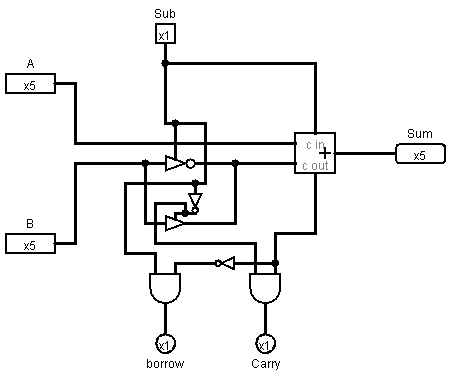
\includegraphics[scale=0.5]{lab4-part1-1.png}
  \item
		2)\\
		So the Adder-Subtracter subtracts B from A (in other words, perform A - B) and in part it does this by inverting the bits in B and adding it to A. However, to make it line up mathematically, you have to add 1 to A.
	\item
		3)\\
    \begin{tabular}{|cc|c||c|} \hline
    A & B & Sub & Sum\\ \hline
    x & y & 0   & $x+y$\\
    x & y & 1   & $x-y$\\ \hline
    \end{tabular}
  \item
		4)\\
	  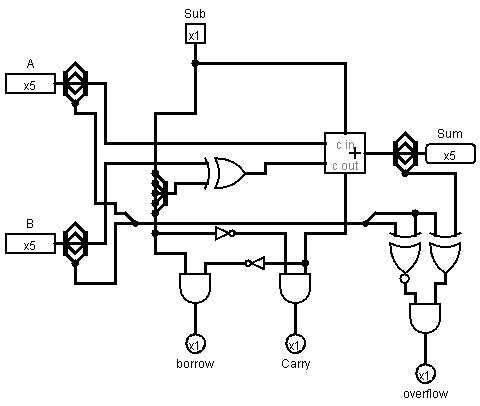
\includegraphics[scale=0.5]{lab4-part1-2.png}
	\item
		5)\\
    \begin{tabular}{|cc|c||c|} \hline
    signA & signB & signSum & overflow\\ \hline
     0 & 0 & 0 & 0 \\
     0 & 0 & 1 & 1 \\
     0 & 1 & 0 & 0 \\
     0 & 1 & 1 & 0 \\
     1 & 0 & 0 & 0 \\
     1 & 0 & 1 & 0 \\
     1 & 1 & 0 & 1 \\
     1 & 1 & 1 & 0 \\ \hline
    \end{tabular}
\end{itemize}
	Part 2 - Two-Port Adder
\begin{itemize}
	\item
		5-bit two-port adder circuit:
	\item
		1)\\
		The Xor gate essentially works like a bitwise inverter when Sub = 1 and like a gate that doesn't change anything when Sub = 0.
	\item
		2)\\
		The wiring of the splitter near the Xor gate takes whatever the value of Sub is and replicates it over 5-bits. So if Sub = 1, then the splitter outputs 11111.
	\item
		3)\\
		There are 5 control bits.
	\item
		4)\\
		Two, Addition and subtraction. I'm not sure what Acc is doing here, its doesn't seem to change anything.
		I can't get the register to change to the input value at all.
	\item
		5)
		By changing the Rmux control signal, one can choose one of the four input. The chosen signal will be added to the register value if Sub = 0, or subtracted from the register value if Sub = 1.
\end{itemize}
\end{document}
